%% 자동 생성. 편집하지 말 것. 생성기: build.py
\PassOptionsToPackage{unicode,hidelinks}{hyperref}
\documentclass[aspectratio=169,10pt]{beamer}
\usepackage{kotex}
\usepackage{fontspec}
\usepackage{graphicx}
\usepackage{tikz}
\usetikzlibrary{positioning,arrows.meta,calc}
\usetheme{default}
\setbeamertemplate{navigation symbols}{}
\setbeamertemplate{footline}{}
\setbeamertemplate{headline}{}
\setbeamercolor{background canvas}{bg=krdsgray0}
\definecolor{krdsprimary5}{HTML}{ECF2FE}
\definecolor{krdsprimary10}{HTML}{D8E5FD}
\definecolor{krdsprimary20}{HTML}{B1CEFB}
\definecolor{krdsprimary30}{HTML}{86AFF9}
\definecolor{krdsprimary40}{HTML}{4C87F6}
\definecolor{krdsprimary50}{HTML}{256EF4}
\definecolor{krdsprimary60}{HTML}{0B50D0}
\definecolor{krdsprimary70}{HTML}{083891}
\definecolor{krdsprimary80}{HTML}{052561}
\definecolor{krdssecondary5}{HTML}{EEF2F7}
\definecolor{krdssecondary10}{HTML}{D6E0EB}
\definecolor{krdssecondary70}{HTML}{063A74}
\definecolor{krdsgray0}{HTML}{FFFFFF}
\definecolor{krdsgray5}{HTML}{F4F5F6}
\definecolor{krdsgray10}{HTML}{E6E8EA}
\definecolor{krdsgray20}{HTML}{CDD1D5}
\definecolor{krdsgray30}{HTML}{B1B8BE}
\definecolor{krdsgray40}{HTML}{8A949E}
\definecolor{krdsgray50}{HTML}{6D7882}
\definecolor{krdsgray60}{HTML}{58616A}
\definecolor{krdsgray70}{HTML}{464C53}
\definecolor{krdsgray80}{HTML}{33363D}
\definecolor{krdsgray90}{HTML}{1E2124}
\definecolor{krdsgray95}{HTML}{131416}
\definecolor{krdsgraphic10}{HTML}{E5ECF9}
\definecolor{krdsgraphic70}{HTML}{39506C}
\definecolor{krdssuccess60}{HTML}{267337}
\definecolor{krdswarning60}{HTML}{8A5C00}
\definecolor{krdsdanger60}{HTML}{BD2C0F}

\setmainfont{PretendardGOV-}[
  Path=/home/campbell/projects/personal/products/malgyeol/artifacts/hackathon/fonts/, Extension=.ttf,
  UprightFont=*Regular, BoldFont=*Bold, ItalicFont=*Regular, BoldItalicFont=*Bold]
\setmainhangulfont{PretendardGOV-}[
  Path=/home/campbell/projects/personal/products/malgyeol/artifacts/hackathon/fonts/, Extension=.ttf,
  UprightFont=*Regular, BoldFont=*Bold, ItalicFont=*Regular, BoldItalicFont=*Bold]
\setsansfont{PretendardGOV-}[
  Path=/home/campbell/projects/personal/products/malgyeol/artifacts/hackathon/fonts/, Extension=.ttf, UprightFont=*Regular, BoldFont=*Bold]
\setsanshangulfont{PretendardGOV-}[
  Path=/home/campbell/projects/personal/products/malgyeol/artifacts/hackathon/fonts/, Extension=.ttf, UprightFont=*Regular, BoldFont=*Bold]
\newhangulfontfamily\krdsfallback{Noto Sans CJK KR}

\hypersetup{colorlinks=true, urlcolor=krdsgray50, pdfborder={0 0 0}}
\setlength{\parindent}{0pt}
\begin{document}

\begin{frame}[plain]
\begin{tikzpicture}[x=1mm,y=1mm,remember picture,overlay,shift={($(current page.center)+(-80.00mm,-45.00mm)$)}]
\node[anchor=north west, text width=30.00mm, align=left, inner sep=0] at (12.00,85.00) {\fontsize{7.6}{11.0}\selectfont\bfseries\color{krdsprimary70}말결};
\node[anchor=north west, text width=70.00mm, align=left, inner sep=0] at (19.36,84.65) {\fontsize{6.4}{9.3}\selectfont\color{krdsgray50}전화 기반 생활지원 연계};
\node[anchor=north west, text width=40.00mm, align=right, inner sep=0] at (108.00,85.00) {\fontsize{6.4}{9.3}\selectfont\color{krdsgray40}서울시 정책 협력 및 현장 실증 제안};
\path[fill=krdsgray10] (12.00,81.80) rectangle (148.00,82.00);
\node[anchor=north west, text width=136.00mm, align=left, inner sep=0] at (12.00,78.40) {\fontsize{7.6}{11.0}\selectfont\bfseries\color{krdsprimary60}01  추진 배경 및 현장 과제};
\node[anchor=north west, text width=136.00mm, align=left, inner sep=0] at (12.00,72.60) {\fontsize{19.0}{27.6}\selectfont\bfseries\color{krdsgray90}\mbox{상담} \mbox{이후} \mbox{반복} \mbox{업무의} \mbox{경감}};
\path[fill=krdsgray5, rounded corners=1.2mm] (12.00,49.00) rectangle (148.00,62.00);
\path[fill=krdsprimary50] (12.00,49.00) rectangle (13.20,62.00);
\node[anchor=north west, text width=13.00mm, align=left, inner sep=0] at (16.20,58.71) {\fontsize{11.0}{15.9}\selectfont\bfseries\color{krdsprimary30}01};
\node[anchor=north west, text width=115.00mm, align=left, inner sep=0] at (29.00,58.39) {\fontsize{10.5}{15.2}\selectfont\color{krdsgray90}\mbox{생활} \mbox{필요·이용} \mbox{조건의} \mbox{반복} \mbox{설명}};
\path[fill=krdsgray5, rounded corners=1.2mm] (12.00,33.00) rectangle (148.00,46.00);
\path[fill=krdsprimary50] (12.00,33.00) rectangle (13.20,46.00);
\node[anchor=north west, text width=13.00mm, align=left, inner sep=0] at (16.20,42.71) {\fontsize{11.0}{15.9}\selectfont\bfseries\color{krdsprimary30}02};
\node[anchor=north west, text width=115.00mm, align=left, inner sep=0] at (29.00,42.39) {\fontsize{10.5}{15.2}\selectfont\color{krdsgray90}\mbox{기관별} \mbox{신청} \mbox{절차·제공} \mbox{조건의} \mbox{분산}};
\path[fill=krdsgray5, rounded corners=1.2mm] (12.00,17.00) rectangle (148.00,30.00);
\path[fill=krdsprimary50] (12.00,17.00) rectangle (13.20,30.00);
\node[anchor=north west, text width=13.00mm, align=left, inner sep=0] at (16.20,26.71) {\fontsize{11.0}{15.9}\selectfont\bfseries\color{krdsprimary30}03};
\node[anchor=north west, text width=115.00mm, align=left, inner sep=0] at (29.00,26.39) {\fontsize{10.5}{15.2}\selectfont\color{krdsgray90}\mbox{기관} \mbox{문의·조건} \mbox{조율·결과} \mbox{회신의} \mbox{연속} \mbox{처리}};
\path[fill=krdsgray20] (12.00,13.40) rectangle (148.00,13.65);
\node[anchor=north west, text width=122.00mm, align=left, inner sep=0] at (12.00,10.80) {\fontsize{5.6}{8.1}\selectfont\color{krdsgray50}출처  \href{https://github.com/sergiobuilds/malgyeol/blob/feat/ai-for-good-product/POLICY\_BASIS.md}{말결 정책·실증 근거}  ·  \href{https://www.seoul.go.kr/news/news\_report.do?nttNo=454831\&srchCtgry=475}{서울형 통합돌봄 시행 발표}};
\node[anchor=north west, text width=12.00mm, align=right, inner sep=0] at (136.00,10.80) {\fontsize{5.6}{8.1}\selectfont\color{krdsgray40}1 / 6};
\end{tikzpicture}
\end{frame}
\begin{frame}[plain]
\begin{tikzpicture}[x=1mm,y=1mm,remember picture,overlay,shift={($(current page.center)+(-80.00mm,-45.00mm)$)}]
\node[anchor=north west, text width=30.00mm, align=left, inner sep=0] at (12.00,85.00) {\fontsize{7.6}{11.0}\selectfont\bfseries\color{krdsprimary70}말결};
\node[anchor=north west, text width=70.00mm, align=left, inner sep=0] at (19.36,84.65) {\fontsize{6.4}{9.3}\selectfont\color{krdsgray50}전화 기반 생활지원 연계};
\node[anchor=north west, text width=40.00mm, align=right, inner sep=0] at (108.00,85.00) {\fontsize{6.4}{9.3}\selectfont\color{krdsgray40}서울시 정책 협력 및 현장 실증 제안};
\path[fill=krdsgray10] (12.00,81.80) rectangle (148.00,82.00);
\node[anchor=north west, text width=136.00mm, align=left, inner sep=0] at (12.00,78.40) {\fontsize{7.6}{11.0}\selectfont\bfseries\color{krdsprimary60}02  지원사업 연계체계};
\node[anchor=north west, text width=136.00mm, align=left, inner sep=0] at (12.00,72.60) {\fontsize{19.0}{27.6}\selectfont\bfseries\color{krdsgray90}\mbox{네} \mbox{사업의} \mbox{기관·관할·이용절차} \mbox{통합}};
\path[fill=krdsgray5, rounded corners=1.2mm] (12.00,42.50) rectangle (77.00,62.00);
\path[fill=krdsprimary50] (12.00,42.50) rectangle (13.20,62.00);
\node[anchor=north west, text width=55.40mm, align=left, inner sep=0] at (17.40,57.80) {\fontsize{10.0}{14.5}\selectfont\bfseries\color{krdsprimary70}\mbox{푸드뱅크·푸드마켓}};
\node[anchor=north west, text width=55.40mm, align=left, inner sep=0] at (17.40,51.28) {\fontsize{9.0}{13.0}\selectfont\color{krdsgray80}\mbox{등록·선정·수령} \mbox{경로}};
\path[fill=krdsgray5, rounded corners=1.2mm] (83.00,42.50) rectangle (148.00,62.00);
\path[fill=krdsprimary50] (83.00,42.50) rectangle (84.20,62.00);
\node[anchor=north west, text width=55.40mm, align=left, inner sep=0] at (88.40,57.80) {\fontsize{10.0}{14.5}\selectfont\bfseries\color{krdsprimary70}\mbox{찾아가는} \mbox{푸드마켓}};
\node[anchor=north west, text width=55.40mm, align=left, inner sep=0] at (88.40,51.28) {\fontsize{9.0}{13.0}\selectfont\color{krdsgray80}\mbox{지역·일정·이용} \mbox{방식}};
\path[fill=krdsgray5, rounded corners=1.2mm] (12.00,17.00) rectangle (77.00,36.50);
\path[fill=krdsprimary50] (12.00,17.00) rectangle (13.20,36.50);
\node[anchor=north west, text width=55.40mm, align=left, inner sep=0] at (17.40,32.30) {\fontsize{10.0}{14.5}\selectfont\bfseries\color{krdsprimary70}\mbox{그냥드림}};
\node[anchor=north west, text width=55.40mm, align=left, inner sep=0] at (17.40,25.78) {\fontsize{9.0}{13.0}\selectfont\color{krdsgray80}\mbox{사업장·준비물·방문} \mbox{절차}};
\path[fill=krdsgray5, rounded corners=1.2mm] (83.00,17.00) rectangle (148.00,36.50);
\path[fill=krdsprimary50] (83.00,17.00) rectangle (84.20,36.50);
\node[anchor=north west, text width=55.40mm, align=left, inner sep=0] at (88.40,32.30) {\fontsize{10.0}{14.5}\selectfont\bfseries\color{krdsprimary70}\mbox{돌봄SOS}};
\node[anchor=north west, text width=55.40mm, align=left, inner sep=0] at (88.40,25.78) {\fontsize{9.0}{13.0}\selectfont\color{krdsgray80}\mbox{거주지} \mbox{접수·돌봄계획·기관} \mbox{의뢰}};
\path[fill=krdsgray20] (12.00,13.40) rectangle (148.00,13.65);
\node[anchor=north west, text width=122.00mm, align=left, inner sep=0] at (12.00,10.80) {\fontsize{5.6}{8.1}\selectfont\color{krdsgray50}출처  \href{https://github.com/sergiobuilds/malgyeol/blob/feat/ai-for-good-product/POLICY\_BASIS.md}{말결 정책·실증 근거}  ·  \href{https://www.s-foodbank.or.kr/intro/intro03}{푸드뱅크·마켓 이용안내}  ·  \href{https://news.seoul.go.kr/welfare/archives/1355}{서울시 찾아가는 푸드마켓 운영}  ·  \href{https://www.s-foodbank.or.kr/justdream/guide}{그냥드림 이용안내}  ·  \href{https://wis.seoul.go.kr/wfs/sos/guide.do}{서울복지포털 돌봄SOS 안내}};
\node[anchor=north west, text width=12.00mm, align=right, inner sep=0] at (136.00,10.80) {\fontsize{5.6}{8.1}\selectfont\color{krdsgray40}2 / 6};
\end{tikzpicture}
\end{frame}
\begin{frame}[plain]
\begin{tikzpicture}[x=1mm,y=1mm,remember picture,overlay,shift={($(current page.center)+(-80.00mm,-45.00mm)$)}]
\node[anchor=north west, text width=30.00mm, align=left, inner sep=0] at (12.00,85.00) {\fontsize{7.6}{11.0}\selectfont\bfseries\color{krdsprimary70}말결};
\node[anchor=north west, text width=70.00mm, align=left, inner sep=0] at (19.36,84.65) {\fontsize{6.4}{9.3}\selectfont\color{krdsgray50}전화 기반 생활지원 연계};
\node[anchor=north west, text width=40.00mm, align=right, inner sep=0] at (108.00,85.00) {\fontsize{6.4}{9.3}\selectfont\color{krdsgray40}서울시 정책 협력 및 현장 실증 제안};
\path[fill=krdsgray10] (12.00,81.80) rectangle (148.00,82.00);
\node[anchor=north west, text width=136.00mm, align=left, inner sep=0] at (12.00,78.40) {\fontsize{7.6}{11.0}\selectfont\bfseries\color{krdsprimary60}03  전화 기반 지원 처리};
\node[anchor=north west, text width=136.00mm, align=left, inner sep=0] at (12.00,72.60) {\fontsize{19.0}{27.6}\selectfont\bfseries\color{krdsgray90}\mbox{AI} \mbox{기관} \mbox{통화와} \mbox{시민} \mbox{회신의} \mbox{연결}};
\node[anchor=north west, text width=136.00mm, align=left, inner sep=0] at (12.00,62.00) {\fontsize{7.4}{10.7}\selectfont\color{krdsgray70}\mbox{업무} \mbox{단위} \mbox{동의와} \mbox{전달} \mbox{정보의} \mbox{제한} \mbox{·} \mbox{기관} \mbox{문의·수령} \mbox{방법} \mbox{조율·신청} \mbox{의사} \mbox{전달} \mbox{·} \mbox{기관} \mbox{답변에} \mbox{따른} \mbox{시민} \mbox{회신·후속} \mbox{연락}};
\path[fill=krdsgraphic10, rounded corners=1.2mm] (12.00,17.00) rectangle (80.00,51.83);
\path[fill=krdsgray0, rounded corners=1.0mm, draw=krdsprimary20, line width=0.2mm] (14.00,47.62) rectangle (78.00,51.23);
\node[anchor=north west, text width=6.00mm, align=left, inner sep=0] at (16.00,51.27) {\fontsize{7.2}{10.4}\selectfont\bfseries\color{krdsprimary50}1};
\node[anchor=north west, text width=56.00mm, align=left, inner sep=0] at (21.00,51.27) {\fontsize{7.2}{10.4}\selectfont\color{krdsgray80}\mbox{시민} \mbox{요청·제약} \mbox{파악}};
\path[fill=krdsgray0, rounded corners=1.0mm, draw=krdsprimary20, line width=0.2mm] (14.00,41.62) rectangle (78.00,45.22);
\node[anchor=north west, text width=6.00mm, align=left, inner sep=0] at (16.00,45.26) {\fontsize{7.2}{10.4}\selectfont\bfseries\color{krdsprimary50}2};
\node[anchor=north west, text width=56.00mm, align=left, inner sep=0] at (21.00,45.26) {\fontsize{7.2}{10.4}\selectfont\color{krdsgray80}\mbox{문의} \mbox{범위} \mbox{동의}};
\path[fill=krdsgray0, rounded corners=1.0mm, draw=krdsprimary20, line width=0.2mm] (14.00,35.61) rectangle (78.00,39.22);
\node[anchor=north west, text width=6.00mm, align=left, inner sep=0] at (16.00,39.26) {\fontsize{7.2}{10.4}\selectfont\bfseries\color{krdsprimary50}3};
\node[anchor=north west, text width=56.00mm, align=left, inner sep=0] at (21.00,39.26) {\fontsize{7.2}{10.4}\selectfont\color{krdsgray80}\mbox{기관} \mbox{발신·조건} \mbox{조율}};
\path[fill=krdsgray0, rounded corners=1.0mm, draw=krdsprimary20, line width=0.2mm] (14.00,29.61) rectangle (78.00,33.21);
\node[anchor=north west, text width=6.00mm, align=left, inner sep=0] at (16.00,33.25) {\fontsize{7.2}{10.4}\selectfont\bfseries\color{krdsprimary50}4};
\node[anchor=north west, text width=56.00mm, align=left, inner sep=0] at (21.00,33.25) {\fontsize{7.2}{10.4}\selectfont\color{krdsgray80}\mbox{답변·후속} \mbox{행동} \mbox{기록}};
\path[fill=krdsgray0, rounded corners=1.0mm, draw=krdsprimary20, line width=0.2mm] (14.00,23.60) rectangle (78.00,27.21);
\node[anchor=north west, text width=6.00mm, align=left, inner sep=0] at (16.00,27.25) {\fontsize{7.2}{10.4}\selectfont\bfseries\color{krdsprimary50}5};
\node[anchor=north west, text width=56.00mm, align=left, inner sep=0] at (21.00,27.25) {\fontsize{7.2}{10.4}\selectfont\color{krdsgray80}\mbox{시민} \mbox{회신·선택}};
\path[fill=krdsgray0, rounded corners=1.0mm, draw=krdsprimary20, line width=0.2mm] (14.00,17.60) rectangle (78.00,21.20);
\node[anchor=north west, text width=6.00mm, align=left, inner sep=0] at (16.00,21.24) {\fontsize{7.2}{10.4}\selectfont\bfseries\color{krdsprimary50}6};
\node[anchor=north west, text width=56.00mm, align=left, inner sep=0] at (21.00,21.24) {\fontsize{7.2}{10.4}\selectfont\color{krdsgray80}\mbox{필요시} \mbox{기관} \mbox{재연락}};
\path[fill=krdsgray5, rounded corners=1.2mm] (84.80,23.61) rectangle (149.20,51.83);
\node[anchor=north west, inner sep=0] at (86.00,50.63) {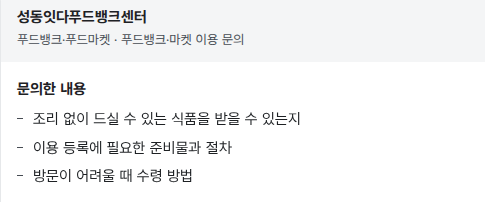
\includegraphics[width=62.00mm,height=25.82mm]{assets/crops/slide3-crop.png}};
\node[anchor=north west, text width=62.00mm, align=left, inner sep=0] at (86.00,22.41) {\fontsize{5.4}{7.8}\selectfont\color{krdsgray50}실제 담당자 화면 · 기관 문의 항목};
\path[fill=krdsgray20] (12.00,13.40) rectangle (148.00,13.65);
\node[anchor=north west, text width=122.00mm, align=left, inner sep=0] at (12.00,10.80) {\fontsize{5.6}{8.1}\selectfont\color{krdsgray50}출처  \href{https://github.com/sergiobuilds/malgyeol/blob/feat/ai-for-good-product/POLICY\_BASIS.md}{말결 정책·실증 근거}  ·  \href{https://github.com/sergiobuilds/malgyeol/blob/feat/ai-for-good-product/dev/active/care-coordination/phone-goal-prompt.md}{말결 전화 구현 계약}  ·  \href{https://github.com/sergiobuilds/malgyeol/blob/feat/ai-for-good-product/dev/active/care-coordination/planning-handoff.md}{말결 계획 인계문}};
\node[anchor=north west, text width=12.00mm, align=right, inner sep=0] at (136.00,10.80) {\fontsize{5.6}{8.1}\selectfont\color{krdsgray40}3 / 6};
\end{tikzpicture}
\end{frame}
\begin{frame}[plain]
\begin{tikzpicture}[x=1mm,y=1mm,remember picture,overlay,shift={($(current page.center)+(-80.00mm,-45.00mm)$)}]
\node[anchor=north west, text width=30.00mm, align=left, inner sep=0] at (12.00,85.00) {\fontsize{7.6}{11.0}\selectfont\bfseries\color{krdsprimary70}말결};
\node[anchor=north west, text width=70.00mm, align=left, inner sep=0] at (19.36,84.65) {\fontsize{6.4}{9.3}\selectfont\color{krdsgray50}전화 기반 생활지원 연계};
\node[anchor=north west, text width=40.00mm, align=right, inner sep=0] at (108.00,85.00) {\fontsize{6.4}{9.3}\selectfont\color{krdsgray40}서울시 정책 협력 및 현장 실증 제안};
\path[fill=krdsgray10] (12.00,81.80) rectangle (148.00,82.00);
\node[anchor=north west, text width=136.00mm, align=left, inner sep=0] at (12.00,78.40) {\fontsize{7.6}{11.0}\selectfont\bfseries\color{krdsprimary60}04  기관 응답별 후속 처리};
\node[anchor=north west, text width=136.00mm, align=left, inner sep=0] at (12.00,72.60) {\fontsize{19.0}{27.6}\selectfont\bfseries\color{krdsgray90}\mbox{필요별} \mbox{진행과} \mbox{중요} \mbox{조건의} \mbox{시민} \mbox{선택}};
\path[fill=krdssecondary5, rounded corners=1.2mm] (12.00,54.40) rectangle (86.00,62.00);
\path[fill=krdssecondary70] (12.00,54.40) rectangle (13.20,62.00);
\node[anchor=north west, text width=12.00mm, align=left, inner sep=0] at (16.20,60.50) {\fontsize{9.0}{13.0}\selectfont\bfseries\color{krdssecondary70}사례};
\node[anchor=north west, text width=55.80mm, align=left, inner sep=0] at (28.20,60.50) {\fontsize{9.0}{13.0}\selectfont\color{krdsgray80}\mbox{조리} \mbox{곤란·생필품} \mbox{필요·방문} \mbox{제약}};
\node[anchor=north west, text width=74.00mm, align=left, inner sep=0] at (12.00,52.40) {\fontsize{7.0}{10.2}\selectfont\bfseries\color{krdsgray60}기관 답변에 따른 갈래};
\path[draw=krdsgray30, line width=0.2mm] (15.00,47.82) -- (15.00,43.28);
\path[draw=krdsgray30, line width=0.2mm, -{Stealth[length=1.0mm]}] (15.00,43.28) -- (18.40,43.28);
\path[fill=krdsgray5, rounded corners=1.2mm] (19.20,38.74) rectangle (86.00,47.82);
\path[fill=krdssuccess60] (19.20,38.74) rectangle (20.40,47.82);
\node[anchor=north west, text width=16.00mm, align=left, inner sep=0] at (23.00,45.58) {\fontsize{8.2}{11.9}\selectfont\bfseries\color{krdssuccess60}유지};
\node[anchor=north west, text width=46.00mm, align=left, inner sep=0] at (39.40,45.58) {\fontsize{8.2}{11.9}\selectfont\color{krdsgray80}\mbox{식사} \mbox{경로} \mbox{유지·생필품} \mbox{대안} \mbox{탐색}};
\path[draw=krdsgray30, line width=0.2mm] (15.00,47.82) -- (15.00,32.41);
\path[draw=krdsgray30, line width=0.2mm, -{Stealth[length=1.0mm]}] (15.00,32.41) -- (18.40,32.41);
\path[fill=krdsgray5, rounded corners=1.2mm] (19.20,27.87) rectangle (86.00,36.94);
\path[fill=krdsprimary60] (19.20,27.87) rectangle (20.40,36.94);
\node[anchor=north west, text width=16.00mm, align=left, inner sep=0] at (23.00,36.80) {\fontsize{8.2}{11.9}\selectfont\bfseries\color{krdsprimary60}재선택};
\node[anchor=north west, text width=46.00mm, align=left, inner sep=0] at (39.40,36.80) {\fontsize{8.2}{11.9}\selectfont\color{krdsgray80}\mbox{비용·일정·수령} \mbox{방법} \mbox{변경} \mbox{시} \mbox{시민} \mbox{재선택}};
\path[draw=krdsgray30, line width=0.2mm] (15.00,47.82) -- (15.00,21.54);
\path[draw=krdsgray30, line width=0.2mm, -{Stealth[length=1.0mm]}] (15.00,21.54) -- (18.40,21.54);
\path[fill=krdsgray5, rounded corners=1.2mm] (19.20,17.00) rectangle (86.00,26.07);
\path[fill=krdswarning60] (19.20,17.00) rectangle (20.40,26.07);
\node[anchor=north west, text width=16.00mm, align=left, inner sep=0] at (23.00,23.83) {\fontsize{8.2}{11.9}\selectfont\bfseries\color{krdswarning60}인계};
\node[anchor=north west, text width=46.00mm, align=left, inner sep=0] at (39.40,23.83) {\fontsize{8.2}{11.9}\selectfont\color{krdsgray80}\mbox{연락} \mbox{이력·남은} \mbox{업무의} \mbox{담당자} \mbox{인계}};
\path[fill=krdsgray5, rounded corners=1.2mm] (90.80,32.45) rectangle (149.20,62.00);
\node[anchor=north west, inner sep=0] at (92.00,60.80) {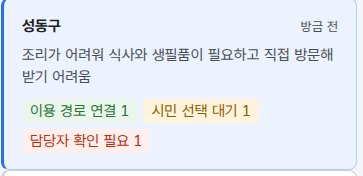
\includegraphics[width=56.00mm,height=27.15mm]{assets/crops/slide4-crop.png}};
\node[anchor=north west, text width=56.00mm, align=left, inner sep=0] at (92.00,31.25) {\fontsize{5.4}{7.8}\selectfont\color{krdsgray50}실제 담당자 화면 · 필요별 진행 상태};
\path[fill=krdsgray20] (12.00,13.40) rectangle (148.00,13.65);
\node[anchor=north west, text width=122.00mm, align=left, inner sep=0] at (12.00,10.80) {\fontsize{5.6}{8.1}\selectfont\color{krdsgray50}출처  \href{https://github.com/sergiobuilds/malgyeol/blob/feat/ai-for-good-product/POLICY\_BASIS.md}{말결 정책·실증 근거}  ·  \href{https://github.com/sergiobuilds/malgyeol/blob/feat/ai-for-good-product/dev/active/care-coordination/planning-handoff.md}{말결 계획 인계문}  ·  \href{https://github.com/sergiobuilds/malgyeol/blob/feat/ai-for-good-product/dev/active/care-coordination/phone-goal-prompt.md}{말결 전화 구현 계약}};
\node[anchor=north west, text width=12.00mm, align=right, inner sep=0] at (136.00,10.80) {\fontsize{5.6}{8.1}\selectfont\color{krdsgray40}4 / 6};
\end{tikzpicture}
\end{frame}
\begin{frame}[plain]
\begin{tikzpicture}[x=1mm,y=1mm,remember picture,overlay,shift={($(current page.center)+(-80.00mm,-45.00mm)$)}]
\node[anchor=north west, text width=30.00mm, align=left, inner sep=0] at (12.00,85.00) {\fontsize{7.6}{11.0}\selectfont\bfseries\color{krdsprimary70}말결};
\node[anchor=north west, text width=70.00mm, align=left, inner sep=0] at (19.36,84.65) {\fontsize{6.4}{9.3}\selectfont\color{krdsgray50}전화 기반 생활지원 연계};
\node[anchor=north west, text width=40.00mm, align=right, inner sep=0] at (108.00,85.00) {\fontsize{6.4}{9.3}\selectfont\color{krdsgray40}서울시 정책 협력 및 현장 실증 제안};
\path[fill=krdsgray10] (12.00,81.80) rectangle (148.00,82.00);
\node[anchor=north west, text width=136.00mm, align=left, inner sep=0] at (12.00,78.40) {\fontsize{7.6}{11.0}\selectfont\bfseries\color{krdsprimary60}05  정책 협력 및 실증 계획};
\node[anchor=north west, text width=136.00mm, align=left, inner sep=0] at (12.00,72.60) {\fontsize{19.0}{27.6}\selectfont\bfseries\color{krdsgray90}\mbox{서울시·자치구} \mbox{협력} \mbox{실증} \mbox{제안}};
\path[fill=krdsgray5, rounded corners=1.2mm] (12.00,42.50) rectangle (77.00,62.00);
\path[fill=krdsprimary50] (12.00,42.50) rectangle (13.20,62.00);
\node[anchor=north west, text width=55.40mm, align=left, inner sep=0] at (17.40,57.80) {\fontsize{10.0}{14.5}\selectfont\bfseries\color{krdsprimary70}\mbox{정책}};
\node[anchor=north west, text width=55.40mm, align=left, inner sep=0] at (17.40,51.28) {\fontsize{9.0}{13.0}\selectfont\color{krdsgray80}\mbox{음성} \mbox{동의·문의·신청} \mbox{보조} \mbox{범위} \mbox{정립}};
\path[fill=krdsgray5, rounded corners=1.2mm] (83.00,42.50) rectangle (148.00,62.00);
\path[fill=krdsprimary50] (83.00,42.50) rectangle (84.20,62.00);
\node[anchor=north west, text width=55.40mm, align=left, inner sep=0] at (88.40,57.80) {\fontsize{10.0}{14.5}\selectfont\bfseries\color{krdsprimary70}\mbox{데이터}};
\node[anchor=north west, text width=55.40mm, align=left, inner sep=0] at (88.40,51.28) {\fontsize{9.0}{13.0}\selectfont\color{krdsgray80}\mbox{네} \mbox{사업의} \mbox{창구·절차·운영정보} \mbox{갱신}};
\path[fill=krdsgray5, rounded corners=1.2mm] (12.00,17.00) rectangle (77.00,36.50);
\path[fill=krdsprimary50] (12.00,17.00) rectangle (13.20,36.50);
\node[anchor=north west, text width=55.40mm, align=left, inner sep=0] at (17.40,32.30) {\fontsize{10.0}{14.5}\selectfont\bfseries\color{krdsprimary70}\mbox{실증환경}};
\node[anchor=north west, text width=55.40mm, align=left, inner sep=0] at (17.40,25.78) {\fontsize{9.0}{13.0}\selectfont\color{krdsgray80}\mbox{참여} \mbox{자치구·기관·문의} \mbox{창구} \mbox{구성}};
\path[fill=krdsgray5, rounded corners=1.2mm] (83.00,17.00) rectangle (148.00,36.50);
\path[fill=krdsprimary50] (83.00,17.00) rectangle (84.20,36.50);
\node[anchor=north west, text width=55.40mm, align=left, inner sep=0] at (88.40,32.30) {\fontsize{10.0}{14.5}\selectfont\bfseries\color{krdsprimary70}\mbox{지원}};
\node[anchor=north west, text width=55.40mm, align=left, inner sep=0] at (88.40,25.78) {\fontsize{9.0}{13.0}\selectfont\color{krdsgray80}\mbox{담당자} \mbox{인계·개인정보} \mbox{검토·측정자료} \mbox{협력}};
\path[fill=krdsgray20] (12.00,13.40) rectangle (148.00,13.65);
\node[anchor=north west, text width=122.00mm, align=left, inner sep=0] at (12.00,10.80) {\fontsize{5.6}{8.1}\selectfont\color{krdsgray50}출처  \href{https://github.com/sergiobuilds/malgyeol/blob/feat/ai-for-good-product/POLICY\_BASIS.md}{말결 정책·실증 근거}  ·  \href{https://www.law.go.kr/LSW/ordinInfoP.do?ordinSeq=2100075}{서울특별시 지역사회 돌봄 통합지원에 관한 조례}  ·  \href{https://www.seoul.go.kr/news/news\_report.do?nttNo=454831\&srchCtgry=475}{서울형 통합돌봄 시행 발표}};
\node[anchor=north west, text width=12.00mm, align=right, inner sep=0] at (136.00,10.80) {\fontsize{5.6}{8.1}\selectfont\color{krdsgray40}5 / 6};
\end{tikzpicture}
\end{frame}
\begin{frame}[plain]
\begin{tikzpicture}[x=1mm,y=1mm,remember picture,overlay,shift={($(current page.center)+(-80.00mm,-45.00mm)$)}]
\node[anchor=north west, text width=30.00mm, align=left, inner sep=0] at (12.00,85.00) {\fontsize{7.6}{11.0}\selectfont\bfseries\color{krdsprimary70}말결};
\node[anchor=north west, text width=70.00mm, align=left, inner sep=0] at (19.36,84.65) {\fontsize{6.4}{9.3}\selectfont\color{krdsgray50}전화 기반 생활지원 연계};
\node[anchor=north west, text width=40.00mm, align=right, inner sep=0] at (108.00,85.00) {\fontsize{6.4}{9.3}\selectfont\color{krdsgray40}서울시 정책 협력 및 현장 실증 제안};
\path[fill=krdsgray10] (12.00,81.80) rectangle (148.00,82.00);
\node[anchor=north west, text width=136.00mm, align=left, inner sep=0] at (12.00,78.40) {\fontsize{7.6}{11.0}\selectfont\bfseries\color{krdsprimary60}06  성과관리 및 추진 방향};
\node[anchor=north west, text width=136.00mm, align=left, inner sep=0] at (12.00,72.60) {\fontsize{19.0}{27.6}\selectfont\bfseries\color{krdsgray90}\mbox{업무부담·연결} \mbox{결과} \mbox{중심의} \mbox{실증} \mbox{평가}};
\path[fill=krdsgray5, rounded corners=1.2mm] (12.00,42.50) rectangle (77.00,62.00);
\path[fill=krdsprimary50] (12.00,42.50) rectangle (13.20,62.00);
\node[anchor=north west, text width=55.40mm, align=left, inner sep=0] at (17.40,57.80) {\fontsize{10.0}{14.5}\selectfont\bfseries\color{krdsprimary70}\mbox{부담} \mbox{지표}};
\node[anchor=north west, text width=55.40mm, align=left, inner sep=0] at (17.40,51.28) {\fontsize{9.0}{13.0}\selectfont\color{krdsgray80}\mbox{요청당} \mbox{통화} \mbox{횟수·담당자} \mbox{처리시간}};
\path[fill=krdsgray5, rounded corners=1.2mm] (83.00,42.50) rectangle (148.00,62.00);
\path[fill=krdsprimary50] (83.00,42.50) rectangle (84.20,62.00);
\node[anchor=north west, text width=55.40mm, align=left, inner sep=0] at (88.40,57.80) {\fontsize{10.0}{14.5}\selectfont\bfseries\color{krdsprimary70}\mbox{연결} \mbox{지표}};
\node[anchor=north west, text width=55.40mm, align=left, inner sep=0] at (88.40,51.28) {\fontsize{9.0}{13.0}\selectfont\color{krdsgray80}\mbox{기관} \mbox{응답시간·필요별} \mbox{결과·회신} \mbox{도달률}};
\path[fill=krdsgray5, rounded corners=1.2mm] (12.00,17.00) rectangle (77.00,36.50);
\path[fill=krdsprimary50] (12.00,17.00) rectangle (13.20,36.50);
\node[anchor=north west, text width=55.40mm, align=left, inner sep=0] at (17.40,32.30) {\fontsize{10.0}{14.5}\selectfont\bfseries\color{krdsprimary70}\mbox{통제} \mbox{지표}};
\node[anchor=north west, text width=55.40mm, align=left, inner sep=0] at (17.40,25.78) {\fontsize{9.0}{13.0}\selectfont\color{krdsgray80}\mbox{중복·취소·권한} \mbox{범위} \mbox{밖} \mbox{실행}};
\path[fill=krdsgray5, rounded corners=1.2mm] (83.00,17.00) rectangle (148.00,36.50);
\path[fill=krdsprimary50] (83.00,17.00) rectangle (84.20,36.50);
\node[anchor=north west, text width=55.40mm, align=left, inner sep=0] at (88.40,32.30) {\fontsize{10.0}{14.5}\selectfont\bfseries\color{krdsprimary70}\mbox{추진} \mbox{과제}};
\node[anchor=north west, text width=55.40mm, align=left, inner sep=0] at (88.40,25.78) {\fontsize{9.0}{13.0}\selectfont\color{krdsgray80}\mbox{기준선} \mbox{측정·협력} \mbox{실증·단계적} \mbox{확대}};
\path[fill=krdsgray20] (12.00,13.40) rectangle (148.00,13.65);
\node[anchor=north west, text width=122.00mm, align=left, inner sep=0] at (12.00,10.80) {\fontsize{5.6}{8.1}\selectfont\color{krdsgray50}출처  \href{https://github.com/sergiobuilds/malgyeol/blob/feat/ai-for-good-product/POLICY\_BASIS.md}{말결 정책·실증 근거}};
\node[anchor=north west, text width=12.00mm, align=right, inner sep=0] at (136.00,10.80) {\fontsize{5.6}{8.1}\selectfont\color{krdsgray40}6 / 6};
\end{tikzpicture}
\end{frame}
\end{document}
